%!TEX root = ../../../adrien_gomar_phd.tex


\begin{figure}[htb]
  \centering
  \subfigure[Low-speed]{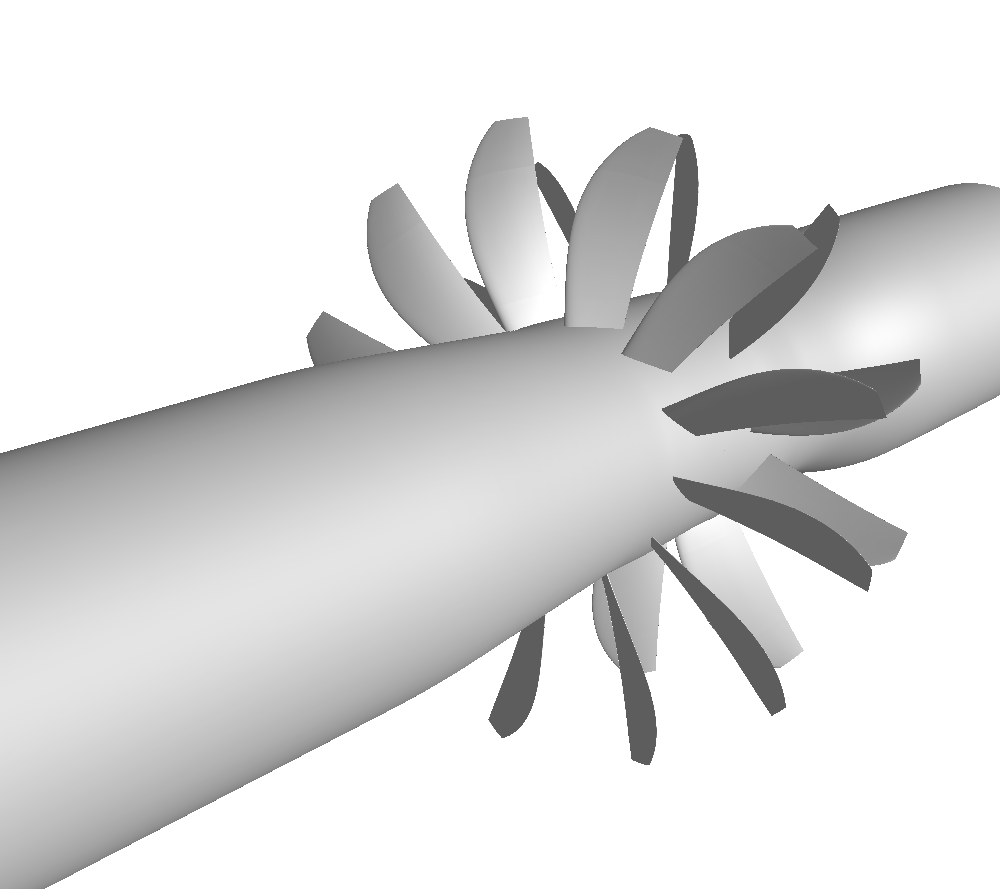
\includegraphics[width=.3\textwidth]{DREAM_LS_wall.png}}
  \subfigure[High-speed]{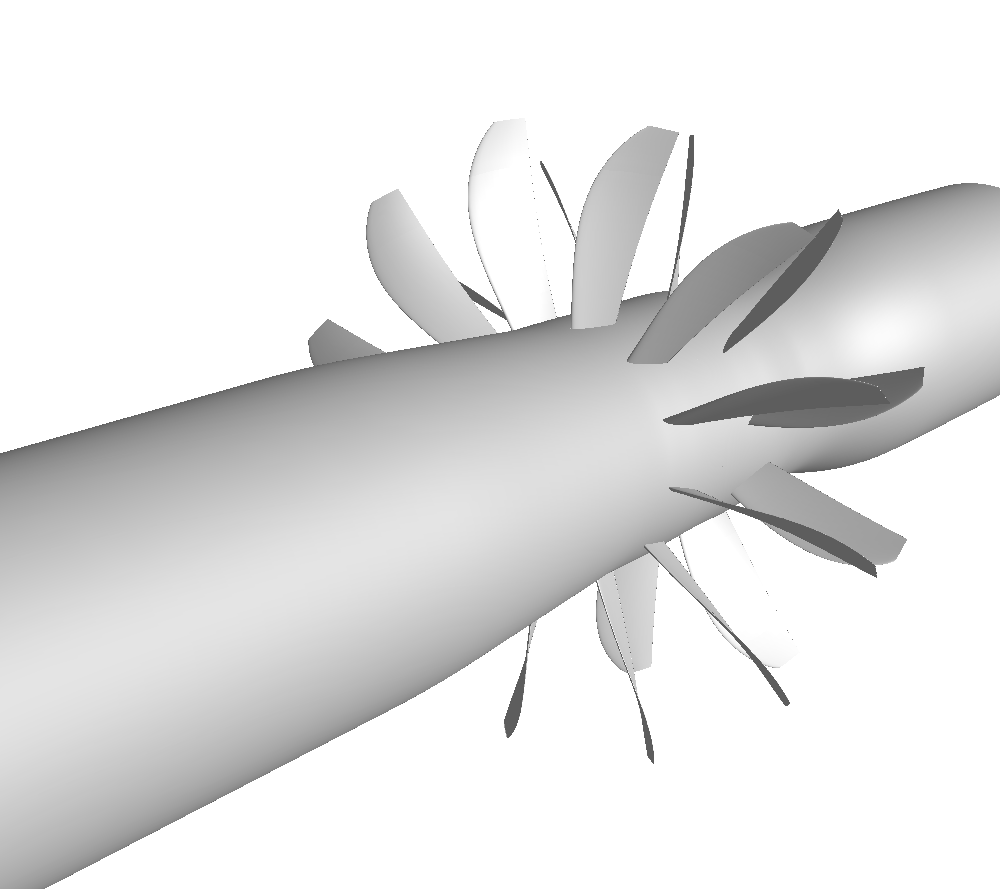
\includegraphics[width=.3\textwidth]{DREAM_HS_wall.png}}
  \caption{DREAM contra-rotating open rotor geometry.}
  \label{fig:dream_wall}
\end{figure}

The DREAM contra-rotating open rotor is shown in Fig.~\ref{fig:dream_wall}
for two flight conditions: Low-Speed (LS) and High-Speed (HS).
These are representative of, respectively, the take-off and
cruise conditions. As one can see in Fig.~\ref{fig:dream_wall},
the pitch angle of the blades is different for the two flight conditions.
This is done to keep a rotation speed almost constant.
\begin{table}[htbp]
  \ra{1.3} \centering
  \begin{tabular}{lcccc}
    \toprule
    \phantom{abdefghijk}& $M_0$ & $|\Omega|$ & $J$ & $M_{tip}$ \\
    \midrule
    Take-off & $0.2$ & $5739~\textrm{tr.min-1}$ & 1.06 & 0.63 \\
    Cruise & $0.73$ & $6057~\textrm{tr.min-1}$ & 3.7 & 0.96  \\
    \bottomrule
  \end{tabular}
  \caption{Flight condition parameters.}
  \label{tab:dream_flight_condition}
\end{table} 
Table~\ref{tab:dream_flight_condition} recalls the main
parameters of the case: the inlet Mach number $M_0$,
the absolute value of the rotation speed of both rotors $|\Omega|$,
the advance ratio $J$ and the Mach number at the tip of
the blade based on the inlet velocity and the advance ratio:
\begin{equation}
	M_{tip} = M_0 \cdot \sqrt{1 + \left(\frac{\pi}{J} \right)^2}
\end{equation}
This equation is a simple transcription of the velocity triangle
applied to the infinite velocity and to the rotation speed perceived
at the front blade tip:
\begin{equation}
    M_{tip} = M_0 \sqrt{1 + \left(\frac{\pi}{J}\right)^2} = 
    \frac{V_0}{\sqrt{\gamma R T_0}} \sqrt{1 + \left(\frac{
    	\cancel{\pi} \cdot \Omega D}{
    	2 \cancel{\pi} \cdot V_0}\right)^2} =
    \sqrt{\frac{V_0^2 + (\Omega R)^2}{\gamma R T_0}}
    \label{eq:m_tip_explained}
\end{equation}
